\chapter{Muon Generation Processes}

Muons with energies above some GeV are naturally produced by cosmic ray or neutrino interactions.
At energies above several TeV, even the strongest accelerator experiments LHC is not powerful enough to create such energetic muons.

At the earths surface most of the muons are going downward, originating from interactions of cosmic ray in the atmosphere.
After $\mathcal{O}(\num{e4})$ meter-water-equivalent (mwe) even the highest energetic muons lost all of their energy and stop before decaying \cite{PDG20}.
Therefore all muons propagating longer distances through the earth will get absorbed.
Only neutrinos can travel through the earth without an interaction and can possibly convert to their charged leptonic counterpart just before the surface.
Therefore muons seen in a detector going downward most-often originate from cosmic rays while upward-going muons originate from neutrino interactions.

\section{Cosmic Ray induced Muons}

Cosmic rays hit the atmosphere with a rate of \SI{1000}{\hertz\per\square\meter} and consist of Protons (\SI{75}{\percent}), Helium (\SI{17}{\percent}) and heavier nuclei \cite{Gaisser16CR}.
Depending on the energy range these ratios are shifted towards the heavier nuclei, mainly iron, dominating at higher energies.
The cosmic ray spectrum is shown in \figref{fig:cr_spectrum} together models describing the composition of the nuclei and the cosmic source classes.

\begin{figure}
    \centering
    \includegraphics[width=\textwidth]{./images/cosmic_ray_spectrum_2.pdf}
    \caption{The energy spectrum of the cosmic rays from the GeV range to the GZK-cutoff. The compositions of the nuclei and on their models describing the all particle spectrum are shown. \cite{Dembinski19MuonPuzzle}}
    \label{fig:cr_spectrum}
\end{figure}

\subsection{Cosmic Ray Energy Spectrum}

The energy spectrum of incoming cosmic rays, shown in \figref{fig:cr_spectrum}, is focusing above the GeV energy range where most of the particles are produced outside of our solar system.
Until energies of roughly a GeV the main source of measured cosmic ray events originate from our sun with a variable event rate depending on the suns activity.
Cosmic rays from outside of our solar system are screened by the Heliosphere.

Above a GeV the magnetic fields of the sun are not powerful enough to accelerate particles to such high energies and galactic sources are the main source of origin.
The main accelerators for the cosmic rays are considered supernova remnants (SNR).
Supernov\ae{} occur in average once in a century in our galaxy, while their shock waves propagate hundreds of years into the interstellar medium.
The particles with these energies are considered to undergo the so called Fermi acceleration, a shock acceleration resulting in a power law spectrum $E^{-\gamma}$ with an index of $\gamma = \num{2}$.
Due to interaction losses and the probability to escape the galactic magnetic field the spectrum gets steeper and results in a measured spectral index of \num{2.7}.
SNRs can accelerate particles up to a PeV, a region called \enquote{knee} of the spectrum.

Above the \enquote{knee} and until the so called \enquote{ankle} at an EeV yet unknown processes, probably Pulsars or Quasars become dominant resulting in an increased measured spectral index of \num{3.1}.
Above the \enquote{ankle} sources inside our galaxy are not powerful enough to accelerate such high energetic particles and extragalactic sources, e.g. Active Galactic Nuclei, become the main contributor.
The resulting spectral shape flattens again to an index of \num{2.6}.
At around \SI{1e20}{eV} the protons interact with the photons of the cosmic microwave Background (CMB) to a Delta resonance, resulting in the GZK-cutoff of the energy spectrum, predicted by Greisen, Zatsepin and Kuz'man \cite{Greisen66GZK, Zatsepin66GZK}.

The CMB is a left-over from the big bang when the temperature drops below the critical value to perform electromagnetic pair production and annihilation.
Due to the expanding universe, the temperature of the CMB is today at \SI{2.7}{K} \cite{PDG20}.

\subsection{Cosmic Ray induced Air Shower} \label{sec:air_shower}

When cosmic rays reach the earth they interact with the dense medium of the atmosphere.
Depending on the energy and the composition the height of the first interaction is at \SIrange{10}{15}{km}.
The secondary particles of this interaction again interact with the atmosphere resulting in a particle cascade or Air shower of thousands or even millions of particles.
These showers can be categorized into a hadronic, muonic and electromagnetic subshowers, that are illustrated in \figref{fig:air_shower_components}.

\begin{figure}
    \centering
    \begin{subfigure}[t]{0.47\textwidth}
        \centering
        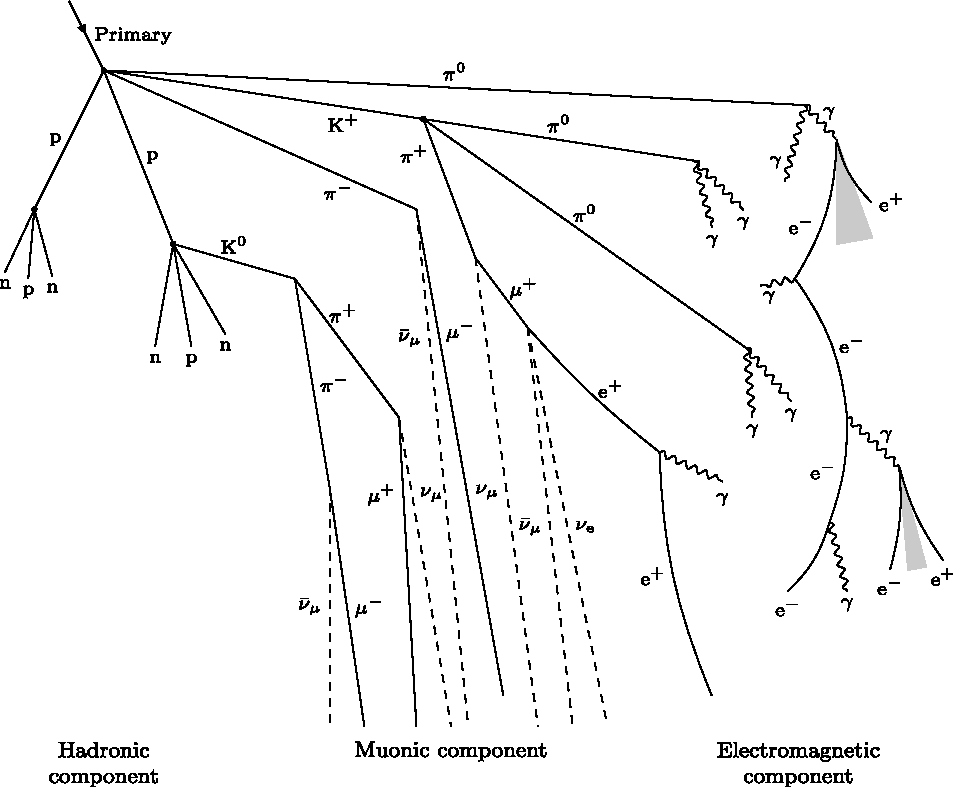
\includegraphics[width=\textwidth]{./images/air_shower_components.pdf}
        \caption{Basic scheme of the shower components of an air shower. \cite{Barrantes18EAS}}
        \label{fig:air_shower_components}
    \end{subfigure}
    \hfill
    \begin{subfigure}[t]{0.47\textwidth}
        \centering
        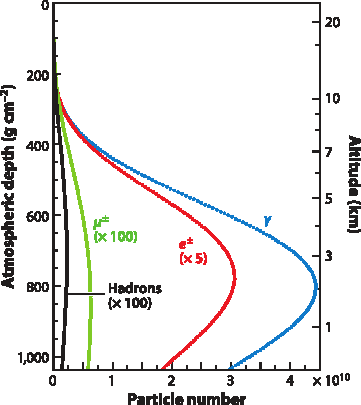
\includegraphics[width=\textwidth]{./images/air_shower_development.pdf}
        \caption{Development of the contribution for the different particles during the air shower. \cite{Engel11EAS}}
        \label{fig:air_shower_development}
    \end{subfigure}
    \caption{Development of a cosmic ray induced air shower. To the left the different sub-showers divided into an electromagnetic, a muonic and a hadronic component is shown. To the right the number of particles during the shower development is shown. Therefore a \SI{e19}{eV} proton induced air shower is simulated.}
    \label{fig:air_shower}
\end{figure}

\textbf{The electromagnetic shower component} consist of electrons, positrons and photons.
Starting e.g. with a high energy photon the two main processes gamma are the production of an electron-positron pair, also called Bethe-Heitler process, and Compton Scattering.
While the latter is just important for the deflection, the pair production is the crucial process for the shower development.
The produced electron or positron dominantly loose their energy via Bremsstrahlung, creating again a high energy photon.
The Positron can also annihilate with the atomic electrons creating a photon pair, which is a sub-dominant process.

(TODO: vgl Tau-Regeneration; wie viel Energie geht in einem cyclus verloren?)
The cylce of photon pair production and electron/positron bremsstrahlung continues until the bremsstrahlung photons are below an MeV and therefore not energetic enough to create an electron/positron pair.
Due to the high number of charged particles (c.f. \figref{fig:air_shower_development}) that are created, this shower component produces the dominant amount of the Cherenkov light and is also important for the radio signal of a shower.
The production of a muon pair is a sub-dominant process as the muon mass is 200 times higher than the electron mass decreasing the phase space and is therefore not important for the em shower development.
Otherwise it is a non-negligible process regarding the number of produced muons inside the shower, while the main production originates from the hadronic shower.

\textbf{The hadronic showercomponent} mainly consist of the lightest mesons, charged Pions and Kaons ($m_{\pi^{\pm}} \approx \SI{140}{MeV}, m_{K^{\pm}} \approx \SI{494}{MeV}$ \cite{PDG20}.
Due to their relatively long lifetimes of $\tau_{\pi^{\pm}} = \SI{26}{ns}$ and $\tau_{K^{\pm}} = \SI{12}{ns}$ they propagate and loose some amount of energy through interactions, before they decay.
Pions decay mainly into muons, as their rest mass is just slightly higher.
Kaons either directly decay into muons or first decay into Pions, which then decay to muons and neutrinos.
The energy losses during the propagation of the Pions and Kaons lead to a steepening of the resulting muon and neutrino energy spectrum with a spectral index of \num{3.7}.
Muons or neutrinos originating from these processes are called \enquote{conventional atmospheric} muons or neutrinos.

Next to Pions and Kaons also short-lived Mesons and baryons occur in hadronic showers.
They consist mainly of mesons with a charm quark, like the D-Meson, of $\Lambda$-Baryons and of unflavored mesons, while the latter do not often decay into muons and muon neutrinos.
Due to their short lifetime, they are not losing energy during their short propagation and directly decay.
The resulting energy spectrum of the decay products therefore remains the same as the primary spectrum and the spectral index does not change.
Although these processes are sub-dominant, the smaller spectral index of the resulting muons and neutrinos makes them relevant at higher energies.
Due of the direct decay of the hadrons, which mainly consist of charmed mesons, the resulting muons or neutrinos are called \enquote{charmed} or \enquote{prompt atmospheric} muons or neutrinos.

\textbf{The muonic showercomponent} mainly originates from the hadronic showercomponent and produce just a few secondaries compared to the other shower particles.
The high muon mass compared to the electron also decreases the interaction probability as the bremsstrahlung cross section is proportinal to $1/m^2$.
Combined with the relatively high lifetime, the muon range through dense media is the highest, neglecting neutrinos, making them the biggest background for all particle detectors even deep underground.
Except of detectors at high altitude, like HAWC \cite{HAWC17} or LHAASO \cite{LHAASO19}, they are the only shower component measured on the earths surface, neglecting the em-radiation part like Cherenkov light, Fluorescence light or the radio signal.

The resulting muon and neutrino energy flux from cosmic ray induced air showers is shown in \figref{fig:atmo_mu_nu_flux}.

\begin{figure}
    \centering
    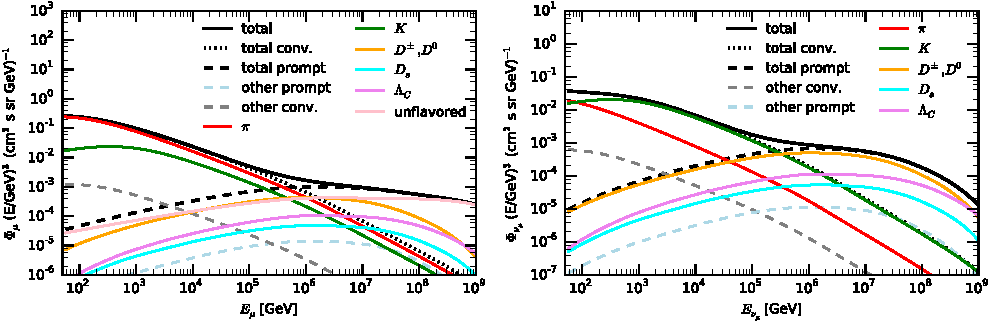
\includegraphics[width=\textwidth]{./images/mceq_mu_nu_flux.pdf}
    \caption{Atmospheric muon and neutrino flux at the surface using MCEq. \cite{Fedynitch15MCEq}}
    \label{fig:atmo_mu_nu_flux}
\end{figure}

A longitudinal shower profile and the contribution of the different sub-shower types is shown in \figref{fig:air_shower_development}.
An increasing number of particles during the beginning of cascade development can be seen as well as a decreasing part when more and more Bremsstrahlung photons are too low energetic for electron pair production.
The resulting maximum of the longitudinal shower profile $X_{\mathrm{max}}$ at roughly \SI{5}{km} varies for the different primary particle types and energies making it an important feature for the primary particle tagging.

Another important feature to estimate the energy of the primary particle is the number of muons detected at the earths surface.
Unfortunately, there is a discrepancy between the number of muons measured in air shower detectors, which exceeds the number of muons produced in air shower simulations starting at primary energies of \SI{e16}{eV}.
by around across multiple experiments with an evidence of \SI{8}{\sigma}, known as the \enquote{Muon Puzzle} \cite{Dembinski19MuonPuzzle}.

A precise description of the muon bundles is also crucial for underground detectors to separate these background events from their signal.
While there are a significant amount of muons with a high transversal momentum resulting in a lateral distribution for the \SI{e19}{eV} event in \figref{fig:air_shower_development} of kilometers \cite{Engel11EAS} most of the high energetic muons propagate close to the primary direction making a separation between them challenging.
An extraction of muon physics parameters out of muon bundles is therefore limited as single muons provide a deeper understanding.

TODO: Plot showing the simulated muon arrival distribution of an air shower on the earths surface.

%
% 
% small seperation between the chapters
%
%

\section{Neutrino induced Muons}

Compared to the cosmic ray induced muons that occur only in bundles, neutrinos produce single muons.
Further muons are produced in the hadronic cascade at the neutrino vertex or as muon pair production.
But these muons have much less energy and stop far before the main muon, so they can be neglected regarding GeV muons or above.

\subsection{Neutrino Energy Spectrum}

The neutrino energy spectrum shown in \figref{fig:neutrino_spectrum} is assumed to starts with a high number of cosmological neutrinos or the cosmic neutrino background (C$\nu$B).
Like the CMB they are left-overs from the big bang when the temperature drops below the critical value of weak lepton production and annihilation.
It consist of all neutrino flavors but the energies are far too low to be measured.

\begin{figure}
    \centering
    \includegraphics[width=\textwidth]{./plots/nu_spectrum.pdf}
    \caption{Neutrino energy spectrum. \cite{KatzSpiering12}}
    \label{fig:neutrino_spectrum}
\end{figure}

At neutrino energies of keV and MeV solar neutrinos from fusion processes dominate the neutrino flux on earth with additional contributions of terrestrial anti-neutrinos from naturally decaying radioactive nuclids.
Additional anti-neutrinos from nuclear reactors also contribute to the neutrino flux depending on the location on earth.
Although only electron neutrinos are produced in radioactive decays or fusion processes, solar neutrinos are measured in all three flavors through the neutrino oscillation further described in section \ref{sec:nu_osc}.

Furthermore in the MeV range neutrinos from supernova remnants also contribute to the neutrino flux.
For the last seen supernova SN1987A, where the neutrino contribution was first measured, the neutrino flux was orders of magnitudes higher than the SNR flux, dominating the spectrum at MeVs during that burst.
% Here the distances are large enough for neutrino oscillation like on every cosmic scale resulting in a neutrino flux of all three flavors.

For neutrino energies starting around a GeV cosmic ray induced atmospheric neutrinos are the main contributors.
Their flux can be approximated by a broken power-law of \enquote{conventional} and \enquote{prompt} atmospheric neutrinos as described in section \ref{sec:air_shower}.
At around \SI{100}{TeV} both the prompt atmospheric and astrophysical neutrinos (probably from AGNs) starts dominating the flux both due to their more flat spectrum.
While the astrophysical flux has already been measured by IceCube, the prompt component has always been fitted to zero and its contribution remain hidden, yet.

The neutrino creation process for the cosmic accelerators (possibly AGNs) is similar to the atmospheric neutrinos.
Accelerated protons interact near the source and through the pion and muon secondaries, neutrinos are produced.
In contrast to the atmospheric neutrinos the medium at astrophysical sources is not as dense as the atmosphere, so the pions and muons do not lose much of their energy before they decay.
Therefore the energy spectrum does not get steeper and the spectral index remains on the level of the Fermi acceleration near 2.

The two main processes of the accelerated protons for the neutrino production are the $pp$-channel and the $p\gamma$-channel.
\begin{align}
    p p \to & \pi^+ \pi^- \dots \\
    p \gamma \to & \Delta^+ \to \begin{cases} \pi^+ n \\ \pi^0 p \end{cases}
\end{align}

In the $pp$-channel a proton interacts with another proton in the surrounding matter near the source producing an equal amount of $\pi^+$ and $\pi^-$.
In the $p\gamma$-channel a proton interacts with a photon producing a Delta-resonance resulting in the production of only positively charged pions.
A way to distinguish between neutrinos and anti-neutrinos at these energies could therefore give further insight of the production processes.

Starting at \SI{10}{PeV} the so called cosmogenic neutrinos are predicted to be the main contributors.
They are produce from decaying Delta-resonances induced by cosmic ray protons at the GZK-limit.
Unfortunately, they have not been measured yet, as the detectors to measure them with radio techniques are currently in the planing and fund raising phase.

\subsection{Neutrino Flavors at Earth} \label{sec:nu_osc}

As already mentioned for solar neutrinos, the primary electron neutrino flux on earth is measured in all three neutrino flavors due to neutrino oscillation \cite{SNO01Oscillation}.
The distance between the earth and the sun is greater than the oscillation length for neutrinos at these energies.
For an initial electron neutrino flux, the oscillations lengths for the lepton flavors are shown in \figref{fig:nu_osc_len}.
Also for terrestrial distances neutrino oscillation is measurable e.g. for atmospheric neutrinos, where the flavor composition depends on the zenith angle \cite{SK98Oscillation}.
The neutrino propagating through the earth further changes due to the different oscillation behavior between the propagation through matter compared to vacuum (MSW effect) \cite{Mikheyev85, Wolfenstein79}.

\begin{figure}
    \centering
    \begin{subfigure}[t]{0.47\textwidth}
        \centering
        \includegraphics[width=\textwidth]{./plots/nu_osc_len.pdf}
        \caption{Oscillation length for an initial electron neutrino flux into the three neutrino flavor.}
        \label{fig:nu_osc_len}
    \end{subfigure}
    \hfill
    \begin{subfigure}[t]{0.47\textwidth}
        \centering
        \includegraphics[width=\textwidth]{./plots/nu_flavor_triangle.pdf}
        \caption{Neutrino flavor triangle for different source scenarios.}
        \label{fig:nu_flavor_trangle}
    \end{subfigure}
    \caption{Neutrino flavor ratios for different observation distances to the source. To the left one full oscillation length is shown and on the right the average of the oscillation periods is shown. The currently measured oscillation parameters \cite{PDG20} and  an inverted mass hierarchy as this is slightly favored is used.}
    \label{fig:nu_osc}
\end{figure}

For astrophysical sources like SNRs or AGNs the propagation distances are much larger than the oscillation length and the mean probability averaged over the oscillation is used to describe the neutrino flux composition depending on the initial production composition.
There are three mainly discussed production scenarios describing a likely and two extreme scenarios of neutrino production.

Assuming pure \textbf{pion decay} processes, the flavor ratio $\nu_e : \nu_{\mu} : \nu_{\tau}$ is $1:2:0$
\begin{align}
    \pi^+ \to &\mu^+ \nu_\mu \\
    &\mu^+ \to e^+ \nu_e \bar{\nu}_{\mu} ,
\end{align}
Equivalent processes happen during the $\pi^-$ decay.

In the \textbf{muon damping} model, also assuming pure pion decays, the produced muons interact near the production region and loose most of their energy before they decay assuming a more dense medium around the source.
The outgoing neutrinos of the muon decay are therefore in the range of a few MeV which is not measurable for astroparticle detectors.
The resulting flavor ratio of $0:1:0$ then does not contain electron neutrinos.
Atmospheric electron neutrinos this leads to the Kaon decay as main production channel as Kaons decay equally into muons and electrons.

In the other extreme scenario a high energetic \textbf{neutron beam} is assumed at the source.
When the neutrons decay, this results in a pure electron neutrino flux and a flavor ratio of $1:0:0$.

For all three neutrino production scenarios the flavor ratio that would be measured on earth after averaging over the neutrino oscillation is shown in \figref{fig:nu_flavor_trangle}.
Independent of the neutrino creation model at the astrophysical source, neutrinos of all three flavors will arrive at the earth through neutrino oscillation, including tau neutrinos.
The most discussed scenario of the dominating pion production without muon damping produces a nearly equal amount of $1:1:1$.

Tau neutrinos are of special interest as the rates to produce the tau lepton with its high mass of \SI{1.7}{GeV} directly is highly suppressed; in air showers or at $pp$ or $p\gamma$ interactions at the source.
They are only measurable through neutrino oscillation and have therefore a high confidence being of astrophysical origin.

Due to the negligible initial tau neutrino flux, the currently measured oscillation parameters assuming the standard model allows the neutrino flavor arriving on earth just to be in a distinct region of the flavor ratio, shown in \figref{fig:nu_flavor_trangle}.
A precise measurement of the neutrino flavors could shrink the allowed source scenarios.

The tau lepton, produced during the neutrino interaction as described in the following section, also decays into muons making them a non-negligible source of neutrino induced muons.

\subsection{Neutrino Interactions}

There are three different interaction modes, illustrated in figure \ref{fig:feyn_nu}, on how neutrinos can interact with matter.
\begin{figure}
    \begin{subfigure}{0.31\textwidth}
        \centering
        %
\begin{tikzpicture}
\begin{feynman}
    % define vertices
    % muon
    \vertex (nu_in) at (-\feynlen, \feynlen);
    \vertex (nu_vertex) at (0, 0.75*\feynlen);
    \vertex[right=2*\feynlen of nu_in] (l_out);
    % nucleus
    \vertex[below=1.5*\feynlen of nu_in] (n_in);
    \vertex[below=\feynlen of nu_vertex] (n_vertex);
    \vertex[below=1.5*\feynlen of l_out] (n_out);
    % draw diagram
    \diagram* {
        (nu_in) -- [fermion] (nu_vertex) -- [fermion] (l_out),
        (nu_vertex) -- [boson, edge label=$W^\mp$] (n_vertex)
    };
    % draw extra features with tikz (not available in tikz-feynman)
    \draw[thick, double] (n_in) -- (n_vertex) -- (n_out);
    \draw[fill] (nu_vertex) circle[radius=\feynvertexsize];
    \draw[fill] (n_vertex) circle[radius=\feynvertexsize];
    % add labels
    \node[left] at (nu_in) {$\nu_{l^\pm}$};
    \node[right] at (l_out) {$l^\pm$};
    \node[left] at (n_in) {$N$};
    \node[right] at (n_out) {$X$};
\end{feynman}
\end{tikzpicture}
%
        \caption{Charged Current (CC)}
        \label{fig:feyn_nu_cc}
    \end{subfigure}
    \hfill
    \begin{subfigure}{0.31\textwidth}
        \centering
        %
\begin{tikzpicture}
\begin{feynman}
    % define vertices
    % muon
    \vertex (nu_in) at (-\feynlen, \feynlen);
    \vertex (nu_vertex) at (0, \feynlen-\feynsmallen);
    \vertex (nu_out) at (\feynlen, \feynlen);
    % nucleus
    \vertex (n_in) at (-\feynlen, -\feynlen);
    \vertex (n_vertex) at (0, -\feynlen+\feynsmallen);
    \vertex (n_out) at (\feynlen, -\feynlen);
    % draw diagram
    \diagram* {
        (nu_in) -- [fermion] (nu_vertex) -- [fermion] (nu_out),
        (nu_vertex) -- [boson] (n_vertex)
    };
    % draw extra features with tikz (not available in tikz-feynman)
    \draw[thick, double] (n_in) -- (n_vertex) -- (n_out);
    \draw[fill] (nu_vertex) circle[radius=\feynvertexsize];
    \draw[fill] (n_vertex) circle[radius=\feynvertexsize];
    % add labels
    \node[left] at (nu_in) {$\nu$};
    \node[right] at (l_out) {$\nu'$};
    \node[right] at (0,0) {$Z^0$};
    \node[left] at (n_in) {$N$};
    \node[right] at (n_out) {$X$};
\end{feynman}
\end{tikzpicture}
%
        \caption{Neutral Current (NC)}
        \label{fig:feyn_nu_nc}
    \end{subfigure}
    \hfill
    \begin{subfigure}{0.31\textwidth}
        \centering
        %
\begin{tikzpicture}
\begin{feynman}
    % define vertices
    \vertex (nu_in) at (-\feynlen, 0.75*\feynlen);
    \vertex (e_in) at (-\feynlen, -0.75*\feynlen);
    \vertex (nu_vertex) at (0, 0);
    \vertex[right=\feynlen of nu_vertex] (w_out);
    % draw diagram
    \diagram* {
        (e_in) -- [fermion] (nu_vertex) -- [fermion] (nu_in),
        (nu_vertex) -- [boson] (w_out)
    };
    % draw extra features with tikz (not available in tikz-feynman)
    \draw[fill] (nu_vertex) circle[radius=\feynvertexsize];
    % add labels
    \node[left] at (nu_in) {$\bar{\nu}_e$};
    \node[left] at (e_in) {$e^-$};
    \node[right] at (w_out) {$W^-$};
\end{feynman}
\end{tikzpicture}
%
        \caption{Glashow Resonance}
        \label{fig:feyn_glashow}
    \end{subfigure}
    \caption{The feynman diagrams of the most dominant neutrino interactions at high energies.}
    \label{fig:feyn_nu}
\end{figure}

The \textbf{Charged Current} (CC) interaction, with a W-Boson as exchange partner between the nucleon and the neutrino, is the main producer of high energy muons.
While the neutrino converts into its charged counterpart-lepton the other outgoing product is the hadronic cascade.
The \textbf{Neutral Current} (NC) Interaction, with an Z-Boson as exchange partner just produces an energy loss of the neutrino without converting it.
Therefore just a hadronic cascade comes out of this interaction as a visible part.
For both the CC and NC interactions in average a third of the neutrino energy is stored as hadronic cascade and two thirds in the outgoing lepton, shown in \figref{fig:nu_xsection_y}.

The CC interaction is the dominant interaction contributing two thirds to the total cross section, while the NC just contribute a third, as shown in \figref{fig:nu_xsection_tot}.
For lower energies the anti neutrino cross section is smaller as the valence quarks are the main interaction partners.
The sea quarks and thereby an equal treatment of neutrino and anti-neutrino become more important at higher energies.

\begin{figure}
    \centering
    \begin{subfigure}[t]{0.47\textwidth}
        \centering
        \includegraphics[width=\textwidth]{./plots/nu_xsection_tot.pdf}
        \caption{Total neutrino cross section}
        \label{fig:nu_xsection_tot}
    \end{subfigure}
    \hfill
    \begin{subfigure}[t]{0.47\textwidth}
        \centering
        \includegraphics[width=\textwidth]{./plots/nu_xsection_average_y.pdf}
        \caption{Average energy loss to the hadronic cascade relative to the neutrino energy.}
        \label{fig:nu_xsection_y}
    \end{subfigure}
    \caption{Neutrino cross section for the Charged Current (CC) the Neutral Current(NC) and the Glashow Resonance(GR). For the CC and NC interaction, the calculation from \cite{CSMS11NuXsection} and for the Glashow resonance, the parametrization of \cite{Barger14} are used.}
    \label{fig:nu_xsection}
\end{figure}

At an energy of \SI{6.3}{PeV} the peak of the \textbf{Glashow Resonance} (GR) dominates the cross section \cite{Glashow60}.
At this energy the anti-electron neutrino interacts resonantly with an atomic electron producing a W-Boson.
The result is a huge hadronic cascade, as the W-Boson decays with the hole energy producing also multiple higher energetic muon tracks characteristic for this interaction.
% The IceCube detector has seen one very likely Glashow-resonance event after 10 years of data taking.

The energy distribution of muons propagating out of a hadronic cascade is shown in \figref{fig:mu_flux_hadr_shower}.
Compared to the directly produced muon of the CC interaction, the secondary muons of the hadronic are much less energetic while still producing a non-negligible signature.
Especially, as the hadronic interactions not only occur at the neutrino vertex, but also at each inelastic nuclear interaction along a muon track.

\begin{figure}
    \centering
    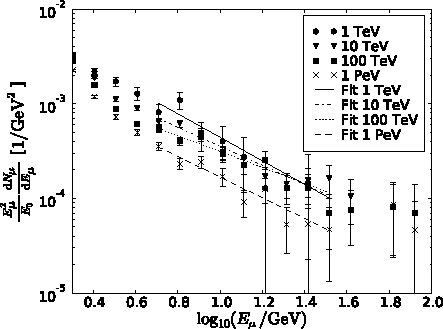
\includegraphics[width=0.8\textwidth]{./images/muon_flux_hadronic_shower.pdf}
    \caption{Differential muon flux for several injected hadronic energies. \cite{Panknin09ICRC}}
    \label{fig:mu_flux_hadr_shower}
\end{figure}
